% -----------------------------------
% -------- BAYSIS - Matched ---------
% -----------------------------------
\subsection{Congestion - Accidents in general}
\label{analysis_processing_correlation_baysis_matched}
The correlation matrix table for the complete congestion-accident matched dataset (see \cref{table:appendix_correlation_matrix_matched_cramers}) is visual presented in \cref{img:correlation_matrix_matched_cramers} showing the the correlation of each variable combination. When visual analyzing \cref{img:correlation_matrix_matched_cramers} and checking the guidelines for a strong correlation in reference to the applied coefficient (identifiable with \cref{table:appendix_coefficient_matrix_matched}) we get a list of strongly correlated variable combinations (see \cref{tbl:correlation_list_baysis_matched}). Since the focus of the thesis are the correlations between accidents and jams, these are only collected from the bottom-left corner of the matrix, where the congestion and accidents variables intersect. Correlations of the kind congestion - congestion or accident - accident are not considered.
\begin{table}[ht!]
	\centering
	\begin{tabular}{c|l}  
		\toprule
		Category & Strong \\
		\midrule
		Str & TMax, TAvg, SMax, SAvg, TDist, SDist, Cov \\ 
 		Kat & TMax, TAvg, SAvg, TDist \\
 		Typ & TDist, Cov \\
 		%Betei & & \\
 		UArt1 & SAvg, TDist, Cov \\ % + SMax
 		%UArt2 & & \\
 		AUrs1 & SAvg, TDist, SDist, Cov, TLHGV \\ % + SMax
 		%AUrs2 & & \\
 		AufHi & TMax, TAvg, TDist, Cov \\
 		%Alkoh & & \\
 		%Char1 & & \\ % -> Strasse
 		%Char2 & & \\
 		%Bes1 & & \\
 		Lich1 & Cov \\
 		Lich2 & Cov \\ % + Lich2
 		Zust1 & Cov \\ % % -> Strasse
 		%Zust2 & & \\
 		%Fstf & & \\ % -> Strasse
 		WoTag & Cov \\
 		%FeiTag & & \\
		Month & Cov \\ % + TMax. SMAx
		\bottomrule
	\end{tabular}
	\caption{List of incident variables and their strong correlated congestion variable from the congestion-accident matched data}
	\label{tbl:correlation_list_baysis_matched}
\end{table}
Next we need to verify that the correlation is significant and what the correlation predicates. Therefore each correlation will be evaluated with the Post Hoc test, defined in \cref{correlation_posthoc}. In the following sections, the correlated relations of the variables in \cref{tbl:correlation_list_baysis_matched} are analyzed and an interpretation of each significant correlation is introduced. Groups with an insufficient sample size (see \cref{correlation_uncertainty}) are neglected and not shown. The descriptive tables, showing the count ($n$), mean ($\bar{x}$), standard deviation ($\sigma$), median ($\tilde{x}$), $min$, $max$ and range ($\Delta$) therefore only contain groups with significant sample sizes.
\begin{figure}[!ht]
	\centering
	\makebox[\textwidth][c]{%
		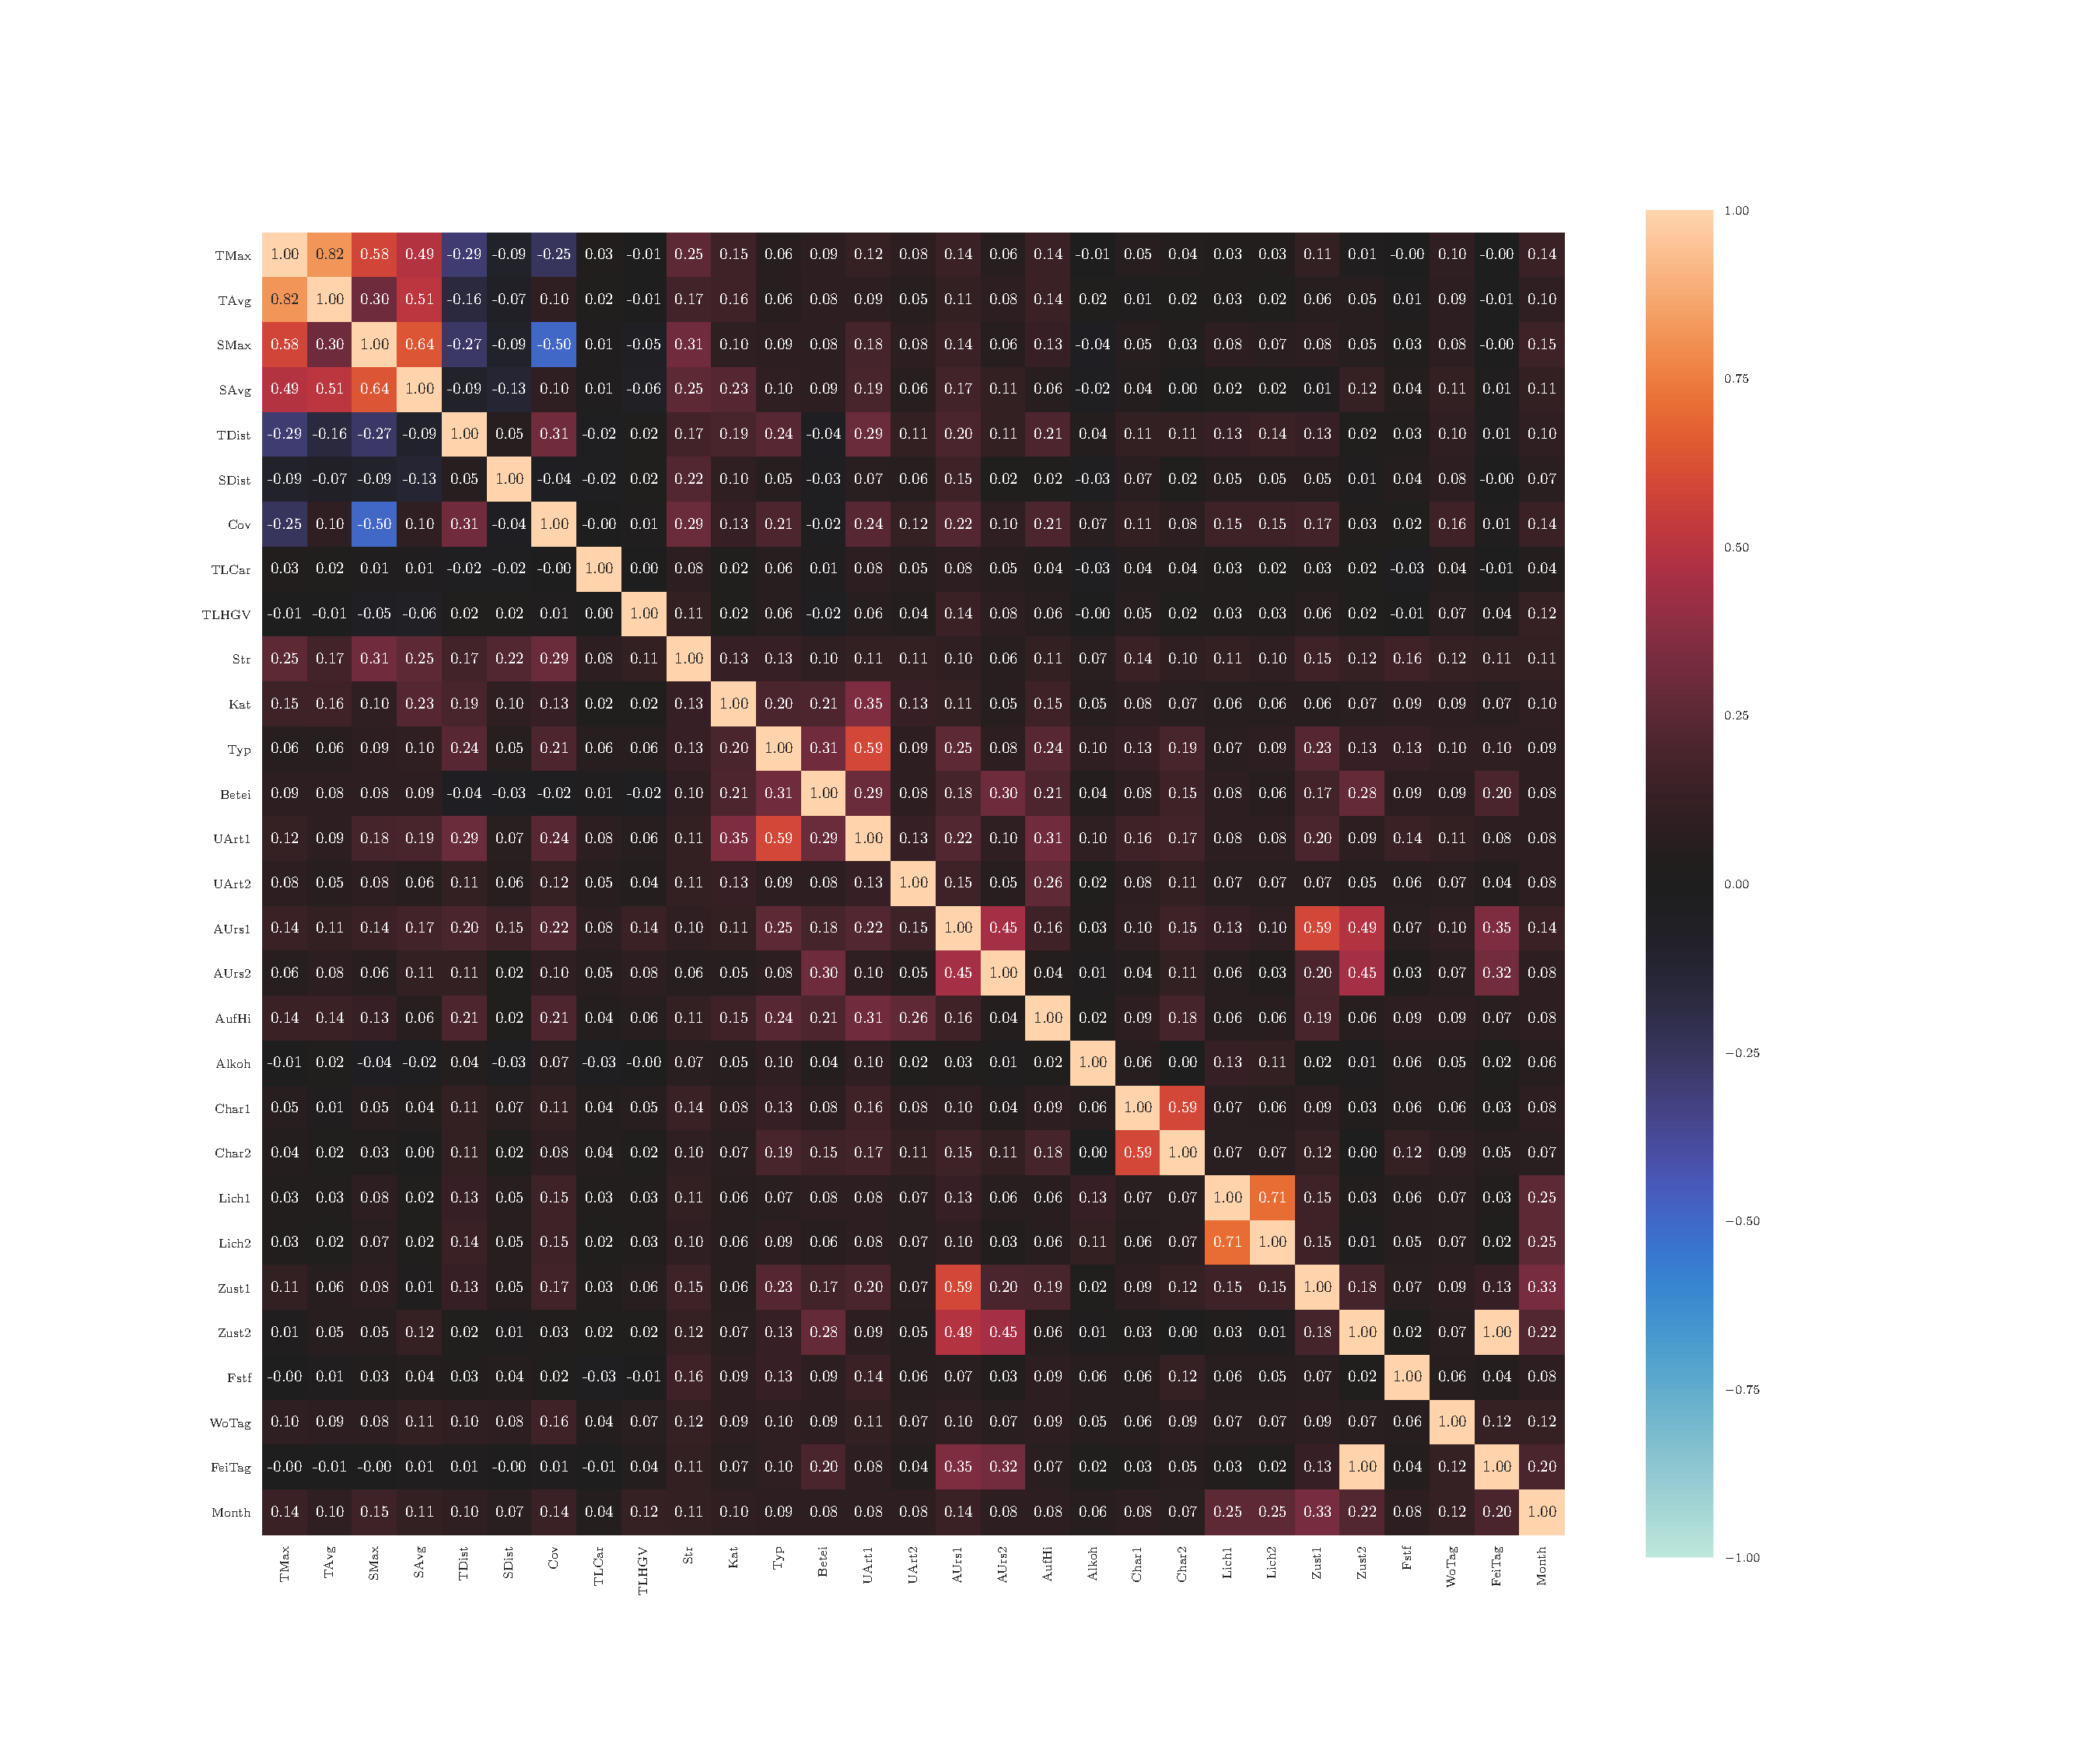
\includegraphics[width=1.4\textwidth, trim=0cm 2.5cm 6cm 3cm]{CorrAnalysis/data/BAYSIS/02_matched/plots/baysis_matched_corr_cramers}%
	}
	\caption{Correlation matrix for congestion-accident matched data calculated with $V$, $\eta$, $\tau$, $r_{pq}$, $r$}
	\label{img:correlation_matrix_matched_cramers}
\end{figure}

% --------------------------
% -------- Strasse ---------
% --------------------------
\centerheading{Street}
This section analyzes the correlated relations of the accident variable \textit{Str}. The correlations of \textit{Str} - \textit{TDist} and \textit{Str} - \textit{SDist} produces a $p$-value above the $\alpha$-level in the Kruskal-Wallis test. The null hypothesis therefore can't be rejected for these relations and there are no significant groups to identify.

The Kruskal-Wallis test of \textit{Str} - \textit{TMax} produces a $p$-value below 0.0001, which is below the $\alpha$-level. The null hypothesis can therefore be rejected, which means that there is a significant difference between the groups of \textit{Str}. To identify the significant groups the pairwise Wilcoxon $T$-test of \textit{Str}-\textit{TMax} produces \cref{tbl:wilcoxon_baysis_matched_Str_TMax}. 
\begin{table}[ht!]
	\tiny
	\setlength{\tabcolsep}{4pt}
	\centering
	\begin{tabular}{rrrrrrrrrrrrrrrrr}
		\toprule
				& A3 & A6 & A9 & A70 & A96 & A7 & A73 & A99 & A92 & A93 & A94 & A72 & A995 & A95 & A71 & A45 \\ 
		\midrule
		% A6 		& 0.00 &  &  &  &  &  &  &  &  &  &  &  &  &  &  &  \\ 
		A9 		& \red{0.01} & 1.00 &  &  &  &  &  &  &  &  &  &  &  &  &  &  \\ 
		A70 	& \red{0.03} & 1.00 & 1.00 &  &  &  &  &  &  &  &  &  &  &  &  &  \\ 
		A96 	& \red{0.00} & 1.00 & 0.27 & 1.00 &  &  &  &  &  &  &  &  &  &  &  &  \\ 
		A7 		& \red{0.00} & 1.00 & 1.00 & 1.00 & 1.00 &  &  &  &  &  &  &  &  &  &  &  \\ 
		A73 	& \red{0.00} & 1.00 & 0.31 & 1.00 & 1.00 & 1.00 &  &  &  &  &  &  &  &  &  &  \\ 
		% A99 	& 1.00 & 1.00 & 1.00 & 1.00 & 0.50 & 1.00 & 0.59 &  &  &  &  &  &  &  &  &  \\ 
		A92 	& \red{0.00} & 1.00 & 0.16 & 1.00 & 1.00 & 1.00 & 1.00 & 0.22 &  &  &  &  &  &  &  &  \\ 
		% A93 	& 1.00 & 1.00 & 1.00 & 1.00 & 1.00 & 1.00 & 1.00 & 1.00 & 1.00 &  &  &  &  &  &  &  \\ 
		A94 	& \red{0.01} & 1.00 & 1.00 & 1.00 & 1.00 & 1.00 & 1.00 & 1.00 & 1.00 & 1.00 &  &  &  &  &  &  \\ 
		% A72 	& 1.00 & 1.00 & 1.00 & 1.00 & 1.00 & 1.00 & 1.00 & 1.00 & 1.00 & 1.00 & 1.00 &  &  &  &  &  \\ 
		% A995 	& 1.00 & 1.00 & 1.00 & 1.00 & 1.00 & 1.00 & 1.00 & 1.00 & 1.00 & 1.00 & 1.00 & 1.00 &  &  &  &  \\ 
		% A95 	& 1.00 & 1.00 & 1.00 & 1.00 & 1.00 & 1.00 & 1.00 & 1.00 & 1.00 & 1.00 & 1.00 & 1.00 & 1.00 &  &  &  \\ 
		% A71 	& 1.00 & 1.00 & 1.00 & 1.00 & 1.00 & 1.00 & 1.00 & 1.00 & 1.00 & 1.00 & 1.00 & 1.00 & 1.00 & 1.00 &  &  \\ 
		% A45 	& 1.00 & 1.00 & 1.00 & 1.00 & 1.00 & 1.00 & 1.00 & 1.00 & 1.00 & 1.00 & 1.00 & 1.00 & 1.00 & 1.00 & 1.00 &  \\ 
		% A980 	& 1.00 & 1.00 & 1.00 & 1.00 & 1.00 & 1.00 & 1.00 & 1.00 & 1.00 & 1.00 & 1.00 & 1.00 & 1.00 & 1.00 & 1.00 & 1.00 \\ 
		\bottomrule
	\end{tabular}
	\caption{Pairwise Wilcoxon $T$-test for \textit{Street} and \textit{Maximal Temporal Extent}}
	\label{tbl:wilcoxon_baysis_matched_Str_TMax}
\end{table}
It shows that the groups A6, A9, A7, A70, A73, A92, A94 and A96 differ from group A3, but is no distinctive general trend.
\begin{table}[ht!]
	\tiny
	\centering
	\begin{tabular}{c|c|c|c|c|c|c|c}
		\toprule
		Group & $n$ & $\bar{x}$ & $\sigma$ & $\tilde{x}$ & $min$ & $max$ & $\Delta$ \\ 
		\midrule
		A3  & 559 & 225.76 & 210.36 & 156.00 & 9  & 1323 & 1314 \\ 
		A6  & 127 & 153.05 & 150.42 & 108.00 & 12 & 864  & 852  \\ 
		A9  & 466 & 170.85 & 151.33 & 118.50 & 9  & 1194 & 1185 \\ 
		A70 & 31  & 106.55 & 79.42  & 81.00  & 24 & 369  & 345  \\ 
		A96 & 155 & 118.32 & 81.05  & 108.00 & 12 & 384  & 372  \\ 
		A7  & 130 & 153.37 & 194.10 & 102.00 & 9  & 1341 & 1332 \\ 
		A73 & 129 & 125.95 & 135.01 & 93.00  & 12 & 1323 & 1311 \\ 
		A99 & 116 & 169.09 & 136.72 & 138.00 & 15 & 681  & 666  \\ 
		A92 & 66  & 103.86 & 65.69  & 87.00  & 18 & 354  & 336  \\ 
		A93 & 21  & 163.57 & 155.71 & 111.00 & 36 & 588  & 552  \\ 
		A94 & 37  & 101.59 & 54.60  & 99.00  & 15 & 249  & 234  \\ 
 		\bottomrule
	\end{tabular}
	\caption{Group descriptives of \textit{Street} and \textit{Maximal Temporal Extent}}
	\label{tbl:descriptives_baysis_matched_Str_TMax}
	%\vspace{-8mm}
\end{table}
The descriptives from \cref{tbl:descriptives_baysis_matched_Str_TMax} show that the mean value of A3 is 27\,\% - 57\,\% higher than the means of A6, A7, A9, A70, A73, A92, and A94. It can be interpreted that accidents on the A3 are associated with significantly longer (temporal) jams than on the A6, A9, A7, A70, A73, A92, and A94. The $\sigma$ supports this interpretation of by $\bar{x}$. The descriptives clearly show three ranked groups of short (A94, A93, A92, A70), medium (A99, A73, A7, A96, A9, A6) and long (A3).

The Kruskal-Wallis test of \textit{Str} - \textit{TAvg} produces a $p$-value of 0.0004, which is below the $\alpha$-level. The null hypothesis can therefore be rejected, which means there is a significant difference between the groups of \textit{Str}. To identify the significant groups the pairwise Wilcoxon $T$-test of \textit{Str}-\textit{TAvg} produces \cref{tbl:wilcoxon_baysis_matched_Str_TAvg}. 
\begin{table}[ht!]
	\tiny
	\setlength{\tabcolsep}{4pt}
	\centering
	\begin{tabular}{rrrrrrrrrrrrrrrrr}
		\toprule
				& A3 & A6 & A9 & A70 & A96 & A7 & A73 & A99 & A92 & A93 & A94 & A72 & A995 & A95 & A71 & A45 \\ 
		\midrule
		% A6 	 & 0.84 &  &  &  &  &  &  &  &  &  &  &  &  &  &  &  \\ 
		% A9 	 & 0.36 & 1.00 &  &  &  &  &  &  &  &  &  &  &  &  &  &  \\ 
		% A70	 & 1.00 & 1.00 & 1.00 &  &  &  &  &  &  &  &  &  &  &  &  &  \\ 
		% A96  & 0.10 & 1.00 & 1.00 & 1.00 &  &  &  &  &  &  &  &  &  &  &  &  \\ 
		% A7 	 & 1.00 & 1.00 & 1.00 & 1.00 & 1.00 &  &  &  &  &  &  &  &  &  &  &  \\ 
		A73  & \red{0.00} & 1.00 & 0.51 & 1.00 & 1.00 & 1.00 &  &  &  &  &  &  &  &  &  &  \\ 
		A99  & \red{0.02} & 1.00 & 1.00 & 1.00 & 1.00 & 1.00 & 1.00 &  &  &  &  &  &  &  &  &  \\ 
		% A92  & 0.26 & 1.00 & 1.00 & 1.00 & 1.00 & 1.00 & 1.00 & 1.00 &  &  &  &  &  &  &  &  \\ 
		% A93  & 1.00 & 1.00 & 1.00 & 1.00 & 1.00 & 1.00 & 1.00 & 1.00 & 1.00 &  &  &  &  &  &  &  \\ 
		% A94  & 0.28 & 1.00 & 1.00 & 1.00 & 1.00 & 1.00 & 1.00 & 1.00 & 1.00 & 1.00 &  &  &  &  &  &  \\ 
		% A72  & 1.00 & 1.00 & 1.00 & 1.00 & 1.00 & 1.00 & 1.00 & 1.00 & 1.00 & 1.00 & 1.00 &  &  &  &  &  \\ 
		% A995 & 1.00 & 1.00 & 1.00 & 1.00 & 1.00 & 1.00 & 1.00 & 1.00 & 1.00 & 1.00 & 1.00 & 1.00 &  &  &  &  \\ 
		% A95  & 1.00 & 1.00 & 1.00 & 1.00 & 1.00 & 1.00 & 1.00 & 1.00 & 1.00 & 1.00 & 1.00 & 1.00 & 1.00 &  &  &  \\ 
		% A71	 & 1.00 & 1.00 & 1.00 & 1.00 & 1.00 & 1.00 & 1.00 & 1.00 & 1.00 & 1.00 & 1.00 & 1.00 & 1.00 & 1.00 &  &  \\ 
		% A45  & 1.00 & 1.00 & 1.00 & 1.00 & 1.00 & 1.00 & 1.00 & 1.00 & 1.00 & 1.00 & 1.00 & 1.00 & 1.00 & 1.00 & 1.00 &  \\ 
		% A980 & 1.00 & 1.00 & 1.00 & 1.00 & 1.00 & 1.00 & 1.00 & 1.00 & 1.00 & 1.00 & 1.00 & 1.00 & 1.00 & 1.00 & 1.00 & 1.00 \\
		\bottomrule
	\end{tabular}
	\caption{Pairwise Wilcoxon $T$-test for \textit{Street} and \textit{Average Temporal Extent}}
	\label{tbl:wilcoxon_baysis_matched_Str_TAvg}
\end{table}
The table shows, that the groups A73 and A99 differ from group A3, but there is no distinctive general trend.
\begin{table}[ht!]
	\tiny
	\centering
	\begin{tabular}{c|c|c|c|c|c|c|c}
		\toprule
		Group & $n$ & $\bar{x}$ & $\sigma$ & $\tilde{x}$ & $min$ & $max$ & $\Delta$ \\  
		\midrule
		A3  & 559 & 89.66 & 98.94  & 65.00 & 4  & 1260 & 1256 \\ 
		A6  & 127 & 69.94 & 65.86  & 56.00 & 3  & 376  & 373  \\ 
		A9  & 466 & 72.92 & 64.55  & 54.00 & 4  & 575  & 571  \\ 
		A70 & 31  & 50.10 & 23.99  & 49.00 & 10 & 99   & 89   \\ 
		A96 & 155 & 61.37 & 44.31  & 52.50 & 5  & 247  & 242  \\ 
		A7  & 130 & 86.55 & 146.82 & 59.50 & 6  & 1326 & 1320 \\ 
		A73 & 129 & 54.78 & 42.48  & 45.00 & 6  & 274  & 268  \\ 
		A99 & 116 & 58.97 & 48.35  & 47.50 & 4  & 295  & 291  \\ 
		A92 & 66  & 55.24 & 36.43  & 51.50 & 8  & 235  & 227  \\ 
		A93 & 21  & 82.33 & 91.10  & 48.00 & 7  & 343  & 336  \\ 
		A94 & 37  & 49.86 & 31.63  & 44.00 & 14 & 145  & 131  \\ 
		\bottomrule
	\end{tabular}
	\caption{Group descriptives for \textit{Street} and \textit{Average Temporal Extent}}
	\label{tbl:descriptives_baysis_matched_Str_TAvg}
	%\vspace{-8mm}
\end{table}
The descriptives from \cref{tbl:descriptives_baysis_matched_Str_TAvg} show that the mean value of A3 is about $\frac{1}{3}$ higher than the means of A73 and A96. We can interpret that accidents on the A3 are associated with significantly longer (temporal) jams than on A73 and A96. The descriptives also show general increase of $\bar{x}$ and $\sigma$ around 35\,\% between the roads A94, A92, A73 and A70 to A3, A6, A7 and A9.

The Kruskal-Wallis test of \textit{Str} - \textit{SMax} produces a $p$-value below 0.0001, which is below the $\alpha$-level. The null hypothesis can therefore be rejected, which means there is a significant difference between the groups of \textit{Str}. To identify the significant groups, a pairwise Wilcoxon $T$-test for \textit{Str} - \textit{SMax} is run, which produces \cref{tbl:wilcoxon_baysis_matched_Str_SMax}.
\begin{table}[ht!]
	\tiny
	\setlength{\tabcolsep}{4pt}
	\centering
	\begin{tabular}{rrrrrrrrrrrrrrrrr}
		\toprule
				& A3   & A6   & A9   & A70  & A96  & A7   & A73   & A99 & A92 & A93 & A94 & A72 & A995 & A95 & A71 & A45 \\ 
		\midrule
		% A6 		& 0.40 &  &  &  &  &  &  &  &  &  &  &  &  &  &  &  \\ 
		A9 		& \red{0.00} & 1.00 &  &  &  &  &  &  &  &  &  &  &  &  &  &  \\ 
		A70 	& \red{0.00} & 0.83 & 0.54 &  &  &  &  &  &  &  &  &  &  &  &  &  \\ 
		A96 	& \red{0.00} & 1.00 & 0.14 & 1.00 &  &  &  &  &  &  &  &  &  &  &  &  \\ 
		A7 		& \red{0.00} & 1.00 & 1.00 & 1.00 & 1.00 &  &  &  &  &  &  &  &  &  &  &  \\ 
		A73 	& \red{0.00} & \red{0.00} & \red{0.00} & 1.00 & 1.00 & 0.59 &  &  &  &  &  &  &  &  &  &  \\ 
		A99 	& 1.00 & 1.00 & 1.00 & 0.80 & 0.31 & 1.00 & \red{0.00} &  &  &  &  &  &  &  &  &  \\ 
		A92 	& \red{0.00} & \red{0.00} & \red{0.00} & 1.00 & 1.00 & 1.00 & 1.00 & \red{0.00} &  &  &  &  &  &  &  &  \\ 
		A93 	& \red{0.03} & 1.00 & 1.00 & 1.00 & 1.00 & 1.00 & 1.00 & 1.00 & 1.00 &  &  &  &  &  &  &  \\ 
		A94 	& \red{0.00} & 0.11 & \red{0.03} & 1.00 & 1.00 & 1.00 & 1.00 & 0.09 & 1.00 & 1.00 &  &  &  &  &  &  \\ 
		% A72 	& 1.00 & 1.00 & 1.00 & 1.00 & 1.00 & 1.00 & 1.00 & 1.00 & 1.00 & 1.00 & 1.00 &  &  &  &  &  \\ 
		% A995 	& 1.00 & 1.00 & 1.00 & 1.00 & 1.00 & 1.00 & 1.00 & 1.00 & 1.00 & 1.00 & 1.00 & 1.00 &  &  &  &  \\ 
		% A95 	& 1.00 & 1.00 & 1.00 & 1.00 & 1.00 & 1.00 & 1.00 & 1.00 & 1.00 & 1.00 & 1.00 & 1.00 & 1.00 &  &  &  \\ 
		% A71 	& 1.00 & 1.00 & 1.00 & 1.00 & 1.00 & 1.00 & 1.00 & 1.00 & 1.00 & 1.00 & 1.00 & 1.00 & 1.00 & 1.00 &  &  \\ 
		% A45 	& 1.00 & 1.00 & 1.00 & 1.00 & 1.00 & 1.00 & 1.00 & 1.00 & 1.00 & 1.00 & 1.00 & 1.00 & 1.00 & 1.00 & 1.00 &  \\ 
		% A980 	& 1.00 & 1.00 & 1.00 & 1.00 & 1.00 & 1.00 & 1.00 & 1.00 & 1.00 & 1.00 & 1.00 & 1.00 & 1.00 & 1.00 & 1.00 & 1.00 \\ 
		\bottomrule
	\end{tabular}
	\caption{Pairwise Wilcoxon $T$-test for \textit{Street} and \textit{Maximal Spatial Extent}}
	\label{tbl:wilcoxon_baysis_matched_Str_SMax}
\end{table}
\cref{tbl:wilcoxon_baysis_matched_Str_SMax} shows, that the groups A7, A9, A70, A73, A92, A94 and A96 differ from group A3. The groups A73 and A92 further differ from group A6 and A9. The group A99 differs from group A73 and group A92 differs from A99, but there is no distinctive general trend.
\begin{table}[ht!]
	\tiny
	\centering
	\begin{tabular}{c|c|c|c|c|c|c|c}
		\toprule
		Group & $n$ & $\bar{x}$ & $\sigma$ & $\tilde{x}$ & $min$ & $max$ & $\Delta$ \\  
		\midrule
		A3  & 559 & 13874.96 & 10064.51 & 11014.00 & 1084 & 46328 & 45244 \\ 
		A6  & 127 & 11067.98 & 8428.07  & 8634.00  & 965  & 43156 & 42191 \\ 
		A9  & 466 & 10680.48 & 7724.45  & 8977.50  & 832  & 49765 & 48933 \\ 
		A70 & 31  & 6676.39  & 3640.24  & 6136.00  & 1841 & 13058 & 11217 \\ 
		A96 & 155 & 8551.75  & 6431.18  & 6238.00  & 971  & 27965 & 26994 \\ 
		A7  & 130 & 9018.27  & 7293.14  & 7051.50  & 1108 & 43244 & 42136 \\ 
		A73 & 129 & 6502.88  & 5033.20  & 5327.00  & 1036 & 33764 & 32728 \\ 
		A99 & 116 & 13244.02 & 11313.27 & 9439.50  & 1280 & 48278 & 46998 \\ 
		A92 & 66  & 6186.80  & 4000.10  & 4936.50  & 1176 & 23291 & 22115 \\ 
		A93 & 21  & 6765.00  & 4403.32  & 5323.00  & 1244 & 16922 & 15678 \\ 
		A94 & 37  & 6220.38  & 3984.46  & 5768.00  & 1167 & 15550 & 14383 \\ 
		\bottomrule
	\end{tabular}
	\caption{Group descriptives of \textit{Street} and \textit{Maximal Spatial Extent}}
	\label{tbl:descriptives_baysis_matched_Str_SMax}
	%\vspace{-8mm}
\end{table}
The descriptives from \cref{tbl:descriptives_baysis_matched_Str_SMax} show that the mean of A3 is 44\,\% - 66\,\% higher than the means of A7, A9, A70, A73, A92, A94 and A96. It also shows that the groups A6, A9 and A99 have a up to 50\,\% higher mean than the groups A73 and A92. We can interpret that accidents on the A3, A6, A9 and A99 are associated with significantly longer (spatial) jams than on A7, A73, A92, A94 and A96. Based on the $\bar{x}$ and $\sigma$ the roads can be separated into three groups of short (A94, A93, A92, A73 and A70), medium (A96 and A7) and long (A3, A6, A9 and A99).

The Kruskal-Wallis test of \textit{Str} - \textit{SAvg} produces a $p$-value of 0.0027, which is below $\alpha=.05$. The null hypothesis can therefore be rejected, which means there is a significant difference between the groups of \textit{Str}. To identify the significant groups, a pairwise Wilcoxon $T$-test for \textit{Str} - \textit{SAvg} is run, which produces \cref{tbl:wilcoxon_baysis_matched_Str_SAvg}.
\begin{table}[ht!]
	\tiny
	\setlength{\tabcolsep}{4pt}
	\centering
	\begin{tabular}{rrrrrrrrrrrrrrrrr}
		\toprule
	 		 & A3 & A6 & A9 & A70 & A96 & A7 & A73 & A99 & A92 & A93 & A94 & A72 & A995 & A95 & A71 & A45 \\ 
		\midrule
		% A6   & 1.00 &  &  &  &  &  &  &  &  &  &  &  &  &  &  &  \\ 
	  	% A9   & 1.00 & 1.00 &  &  &  &  &  &  &  &  &  &  &  &  &  &  \\ 
	  	A70  & \red{0.05} & 0.83 & 0.71 &  &  &  &  &  &  &  &  &  &  &  &  &  \\ 
	  	A96  & \red{0.05} & 1.00 & 1.00 & 1.00 &  &  &  &  &  &  &  &  &  &  &  &  \\ 
	  	% A7   & 1.00 & 1.00 & 1.00 & 1.00 & 1.00 &  &  &  &  &  &  &  &  &  &  &  \\ 
	  	A73  & \red{0.00} & \red{0.00} & \red{0.00} & 1.00 & \red{0.00} & \red{0.00} &  &  &  &  &  &  &  &  &  &  \\ 
	  	A99  & \red{0.00} & 1.00 & 0.06 & 1.00 & 1.00 & 1.00 & 0.51 &  &  &  &  &  &  &  &  &  \\ 
	  	A92  & \red{0.00} & 0.61 & \red{0.03} & 1.00 & 1.00 & 1.00 & 1.00 & 1.00 &  &  &  &  &  &  &  &  \\ 
	  	A93  & \red{0.03} & 0.46 & 0.16 & 1.00 & 1.00 & 1.00 & 1.00 & 1.00 & 1.00 &  &  &  &  &  &  &  \\ 
	  	A94  & \red{0.00} & 0.07 & 0.01 & 1.00 & 0.36 & 0.31 & 1.00 & 1.00 & 1.00 & 1.00 &  &  &  &  &  &  \\ 
	  	% A72  & 1.00 & 1.00 & 1.00 & 1.00 & 1.00 & 1.00 & 1.00 & 1.00 & 1.00 & 1.00 & 1.00 &  &  &  &  &  \\ 
	  	% A995 & 1.00 & 1.00 & 1.00 & 1.00 & 1.00 & 1.00 & 1.00 & 1.00 & 1.00 & 1.00 & 1.00 & 1.00 &  &  &  &  \\ 
	  	% A95  & 1.00 & 1.00 & 1.00 & 1.00 & 1.00 & 1.00 & 1.00 & 1.00 & 1.00 & 1.00 & 1.00 & 1.00 & 1.00 &  &  &  \\ 
	  	% A71  & 1.00 & 1.00 & 1.00 & 1.00 & 1.00 & 1.00 & 1.00 & 1.00 & 1.00 & 1.00 & 1.00 & 1.00 & 1.00 & 1.00 &  &  \\ 
	  	% A45  & 1.00 & 1.00 & 1.00 & 1.00 & 1.00 & 1.00 & 1.00 & 1.00 & 1.00 & 1.00 & 1.00 & 1.00 & 1.00 & 1.00 & 1.00 &  \\ 
	  	% A980 & 1.00 & 1.00 & 1.00 & 1.00 & 1.00 & 1.00 & 1.00 & 1.00 & 1.00 & 1.00 & 1.00 & 1.00 & 1.00 & 1.00 & 1.00 & 1.00 \\ 
		\bottomrule
	\end{tabular}
	\caption{Pairwise Wilcoxon $T$-test for \textit{Street} and \textit{Average Spatial Extent}}
	\label{tbl:wilcoxon_baysis_matched_Str_SAvg}
\end{table}
\cref{tbl:wilcoxon_baysis_matched_Str_SAvg} shows, that the groups A70, A73, A92, A93, A94, A96 and A99 differ from group A3. The groups A73, A94 further differ from group A6 as well as A73, A99, A92 and A94 from group A9, but there is no distinctive general trend.
\begin{table}[ht!]
	\tiny
	\centering
	\begin{tabular}{c|c|c|c|c|c|c|c}
	  	\toprule
	 	Group & $n$ & $\bar{x}$ & $\sigma$ & $\tilde{x}$ & $min$ & $max$ & $\Delta$ \\  
	  	\midrule
		A3  & 559 & 4537.56 & 2735.62 & 3986.00 & 135  & 17805 & 17670 \\ 
	  	A6  & 127 & 4361.50 & 3042.71 & 3235.00 & 458  & 16851 & 16393 \\ 
	  	A9  & 466 & 4187.15 & 2569.83 & 3700.50 & 393  & 15132 & 14739 \\ 
	  	A70 & 31  & 3010.45 & 2067.63 & 1974.00 & 1008 & 9937  & 8929 \\ 
	  	A96 & 155 & 3678.39 & 2172.99 & 3299.00 & 387  & 10182 & 9795 \\ 
	  	A7  & 130 & 4141.68 & 3026.58 & 3537.50 & 643  & 16571 & 15928 \\ 
	  	A73 & 129 & 2683.97 & 1981.91 & 2232.00 & 544  & 11832 & 11288 \\ 
	  	A99 & 116 & 3240.97 & 1878.87 & 2978.00 & 583  & 8426  & 7843 \\ 
	  	A92 & 66  & 2926.15 & 1521.59 & 2931.50 & 455  & 8970  & 8515 \\ 
	  	A93 & 21  & 2525.43 & 1443.21 & 2338.00 & 664  & 6779  & 6115 \\ 
	  	A94 & 37  & 2691.68 & 2023.38 & 2307.00 & 358  & 10393 & 10035 \\ 
	   	\bottomrule
	\end{tabular}
	\caption{Group descriptives of \textit{Street} and \textit{Average Spatial Extent}}
	\label{tbl:descriptives_baysis_matched_Str_SAvg}
	%\vspace{-8mm}
\end{table}
The descriptives from \cref{tbl:descriptives_baysis_matched_Str_SAvg} show that the mean of A3 is 45\,\% - 55\,\% higher the means of A70, A73, A92, A93, A94, A96 and A99. It also shows that the means of the groups A6, A9 and A99 is about 30\,\% higher mean than the groups A73 and A94. We can interpret that accidents on the A3, A6, A9 and A99 lead are associated with significantly longer (spatial) jams than on A70, A73, A92, A93, A94, A96 and A99. The groups can be separated into two groups based on $\bar{x}$ and $\sigma$. A3, A6, A9 and A7 tend to have longer (spatial) longer jams when A70, A96, A73, A99, A92, A93 and A94 tend to have shorter (spatial) jams.

The Kruskal-Wallis test of \textit{Str} - \textit{Cov} produces a $p$-value of 0.0018, which is below the $\alpha$-level. The null hypothesis can therefore be rejected, which means there is a significant difference between the groups of \textit{Str}. To identify the significant groups, a pairwise Wilcoxon $T$-test for \textit{Str} - \textit{Cov} is run, which produces \cref{tbl:wilcoxon_baysis_matched_Str_Cov}. 
\begin{table}[ht!]
	\tiny
	\setlength{\tabcolsep}{4pt}
	\centering
	\begin{tabular}{rrrrrrrrrrrrrrrrr}
	  	\toprule
				& A3   & A6   & A9   & A70  & A96  & A7   & A73 & A99 & A92 & A93 & A94 & A72 & A995 & A95 & A71 & A45 \\ 
	  	\midrule
		A6 		& \red{0.05} &  &  &  &  &  &  &  &  &  &  &  &  &  &  &  \\ 
	  	A9 		& \red{0.00} & 1.00 &  &  &  &  &  &  &  &  &  &  &  &  &  &  \\ 
	  	% A70 	& 1.00 & 1.00 & 1.00 &  &  &  &  &  &  &  &  &  &  &  &  &  \\ 
	  	A96 	& \red{0.00} & 1.00 & \red{0.00} & 1.00 &  &  &  &  &  &  &  &  &  &  &  &  \\ 
	  	A7 		& \red{0.00} & 1.00 & \red{0.01} & 1.00 & 1.00 &  &  &  &  &  &  &  &  &  &  &  \\ 
	  	A73 	& \red{0.04} & 1.00 & 1.00 & 1.00 & 1.00 & 1.00 &  &  &  &  &  &  &  &  &  &  \\ 
	  	A99 	& 0.88 & \red{0.00} & \red{0.00} & 0.09 & \red{0.00} & \red{0.00} & \red{0.00} &  &  &  &  &  &  &  &  &  \\ 
	  	A92 	& \red{0.00} & 1.00 & 0.12 & 1.00 & 1.00 & 1.00 & 1.00 & \red{0.00} &  &  &  &  &  &  &  &  \\ 
	  	% A93 	& 1.00 & 1.00 & 1.00 & 1.00 & 1.00 & 1.00 & 1.00 & 1.00 & 1.00 &  &  &  &  &  &  &  \\ 
	  	% A94 	& 1.00 & 1.00 & 1.00 & 1.00 & 1.00 & 1.00 & 1.00 & 0.13 & 1.00 & 1.00 &  &  &  &  &  &  \\ 
	  	% A72 	& 1.00 & 1.00 & 1.00 & 1.00 & 1.00 & 1.00 & 1.00 & 1.00 & 1.00 & 1.00 & 1.00 &  &  &  &  &  \\ 
	  	% A995 	& 1.00 & 1.00 & 1.00 & 1.00 & 1.00 & 1.00 & 1.00 & 1.00 & 1.00 & 1.00 & 1.00 & 1.00 &  &  &  &  \\ 
	  	% A95 	& 1.00 & 1.00 & 1.00 & 1.00 & 1.00 & 1.00 & 1.00 & 1.00 & 1.00 & 1.00 & 1.00 & 1.00 & 1.00 &  &  &  \\ 
	  	% A71 	& 1.00 & 1.00 & 1.00 & 1.00 & 1.00 & 1.00 & 1.00 & 1.00 & 1.00 & 1.00 & 1.00 & 1.00 & 1.00 & 1.00 &  &  \\ 
	  	% A45 	& 1.00 & 1.00 & 1.00 & 1.00 & 1.00 & 1.00 & 1.00 & 1.00 & 1.00 & 1.00 & 1.00 & 1.00 & 1.00 & 1.00 & 1.00 &  \\ 
	  	% A980 	& 1.00 & 1.00 & 1.00 & 1.00 & 1.00 & 1.00 & 1.00 & 1.00 & 1.00 & 1.00 & 1.00 & 1.00 & 1.00 & 1.00 & 1.00 & 1.00 \\ 
	   	\bottomrule
	\end{tabular}
	\caption{Pairwise Wilcoxon $T$-test for \textit{Street} and \textit{Coverage}}
	\label{tbl:wilcoxon_baysis_matched_Str_Cov}
\end{table}
\cref{tbl:wilcoxon_baysis_matched_Str_SAvg} shows, that the groups A6, A7, A9, A73, A92 and A96 differ from group A3. The group A99 differs from group A6 and groups A96, AA7, A99, A92 differ from group A9. The group A99 also differs from the groups A70, A96, A7 and A73, but there is no distinctive general trend. 
\begin{table}[ht!]
	\tiny
	\centering
	\begin{tabular}{c|c|c|c|c|c|c|c}
	  	\toprule
	 	Group & $n$ & $\bar{x}$ & $\sigma$ & $\tilde{x}$ & $min$ & $max$ & $\Delta$ \\   
	  	\midrule
		A3  & 559 & 38.44 & 19.04 & 36.00 & 2  & 100 & 98 \\ 
	  	A6  & 127 & 46.99 & 24.06 & 44.00 & 9  & 100 & 91 \\ 
	  	A9  & 466 & 43.93 & 18.49 & 41.00 & 6  & 100 & 94 \\ 
	  	A70 & 31  & 50.29 & 25.00 & 44.00 & 9  & 92  & 83 \\ 
	  	A96 & 155 & 51.94 & 21.38 & 54.00 & 2  & 100 & 98 \\ 
	  	A7  & 130 & 53.46 & 24.19 & 54.00 & 6  & 100 & 94 \\ 
	  	A73 & 129 & 46.49 & 22.88 & 42.00 & 7  & 100 & 93 \\ 
	  	A99 & 116 & 33.21 & 18.03 & 31.00 & 5  & 85  & 80 \\ 
	  	A92 & 66  & 53.15 & 21.80 & 52.50 & 14 & 98  & 84 \\ 
	  	A93 & 21  & 40.81 & 17.72 & 37.00 & 13 & 70  & 57 \\ 
	  	A94 & 37  & 47.76 & 23.69 & 44.00 & 11 & 88  & 77 \\ 	
	  	\bottomrule
	\end{tabular}
	\caption{Group descriptives of \textit{Street} and \textit{Coverage}}
	\label{tbl:descriptives_baysis_matched_Str_Cov}
	%\vspace{-8mm}
\end{table}
The descriptives from \cref{tbl:descriptives_baysis_matched_Str_Cov} show that the mean of A3 is 20\,\% - 30\,\% lower than the means of A6, A7, A9, A73, A92 and A96. It also shows that the mean of A6 is about $\frac{1}{3}$ higher than the mean of A99. We can interpret that accidents on the A3, A99 are associated with significantly less denser jams than on A6, A7, A9, A73, A70, A92 and A96.

% ----------------------
% -------- Kat ---------
% ----------------------
\centerheading{Kat}
\label{ana:baysis_global_Kat}
This section analyzes the correlated relations of the accident variable \textit{Kat}. The encoding and description of the variable \textit{Typ} is shown in \cref{tbl:baysis_dataset_Typ}. The Kruskal-Wallis rank sum test of \textit{Kat} - \textit{SAvg} produces a $p$-value above $\alpha$. The null hypothesis can't be rejected and there is no significant difference between the groups of \textit{Kat} in this relation.

The Kruskal-Wallis test of \textit{Kat} - \textit{TMax} produces a $p$-value of 0.0068, which is below $\alpha=.05$. The null hypothesis can therefore be rejected, which means there is a significant difference between the groups of \textit{Kat}. To identify the significant groups, a pairwise Wilcoxon $T$-test for \textit{Kat} - \textit{TMax} is run, which produces \cref{tbl:wilcoxon_baysis_matched_Kat_TMax}.
\begin{table}[ht!]
	\tiny
	\centering
	\begin{tabular}{rrrr}
	  	\toprule
	 	& 1 & 2 & 3 \\ 
	  	\midrule
		2 & \red{0.00} &  &  \\ 
	  	3 & \red{0.00} & \red{0.01} &  \\ 
	  	7 & \red{0.00} & \red{0.02} & 0.78 \\ 
	   	\bottomrule
	\end{tabular}
	\caption{Pairwise Wilcoxon $T$-test for \textit{Kat} and \textit{Maximal Temporal Extent}}
	\label{tbl:wilcoxon_baysis_matched_Kat_TMax}
\end{table}
\cref{tbl:wilcoxon_baysis_matched_Kat_TMax} shows that all groups, besides of group 7 to group 3, have significant differences. 
\begin{table}[ht!]
	\tiny
	\centering
	\begin{tabular}{c|c|c|c|c|c|c|c}
		\toprule
		Group & $n$ & $\bar{x}$ & $\sigma$ & $\tilde{x}$ & $min$ & $max$ & $\Delta$ \\   
	  	\midrule
		1 & 36  & 317.67 & 215.10 & 279 & 27 & 987  & 960 \\ 
	  	2 & 216 & 189.03 & 164.93 & 135 & 9  & 1257 & 1248 \\ 
	  	3 & 881 & 155.26 & 141.87 & 111 & 9  & 1323 & 1314 \\ 
	  	7 & 718 & 179.35 & 192.33 & 117 & 9  & 1341 & 1332 \\ 
	   	\bottomrule
	\end{tabular}
	\caption{Group descriptives of \textit{Kat} and \textit{Maximal Temporal Extent}}
	\label{tbl:descriptives_baysis_matched_Kat_TMax}
	%\vspace{-8mm}
\end{table}
% 189+155+179 / 3 = 174
% diff 317,174 = 143
% mean diff 189,155,179 = 29
The descriptives from \cref{tbl:descriptives_baysis_matched_Kat_TMax} present increasing means from lightly injured to deathly accident. We can interpret that the maximal temporal jam length  increases with the gravity of the accident. Also the difference of group 1 to group 2, 3 and 7 is quite substantial, which means that the accidents with deaths are associated with 143\,min longer jams, than others. The group of accidents with property damage does significantly differ from the others, but does not fit into the trend. A comparisons of means puts the property damage group in-between of accidents with slightly and heavily injured. The groups 2, 3 and 7 differ by 29\,min on average.

The Kruskal-Wallis test of \textit{Kat} - \textit{TAvg} produces a $p$-value of 0.0005, which is below $\alpha$. The null hypothesis can therefore be rejected, which means there is a significant difference between the groups of \textit{Kat}. To identify the significant groups, a pairwise Wilcoxon $T$-test for \textit{Kat} - \textit{TAvg} is run, which produces \cref{tbl:wilcoxon_baysis_matched_Kat_TAvg}.
\begin{table}[ht!]
	\tiny
	\centering
	\begin{tabular}{rrrr}
	  	\toprule
	 	& 1 & 2 & 3 \\ 
	  	\midrule
		2 & \red{0.00} &  &  \\ 
	  	3 & \red{0.00} & \red{0.00} &  \\ 
	  	7 & \red{0.00} & \red{0.00} & \red{0.05} \\ 
	   	\bottomrule
	\end{tabular}
	\caption{Pairwise Wilcoxon $T$-test for \textit{Kat} and \textit{Average Temporal Extent}}
	\label{tbl:wilcoxon_baysis_matched_Kat_TAvg}
\end{table}
\cref{tbl:wilcoxon_baysis_matched_Kat_TAvg} shows that all groups have significant differences. The descriptives from \cref{tbl:descriptives_baysis_matched_Kat_TAvg} present increasing means from group 3 to 1.
\begin{table}[ht!]
	\tiny
	\centering
	\begin{tabular}{c|c|c|c|c|c|c|c}
	  	\toprule
		Group & $n$ & $\bar{x}$ & $\sigma$ & $\tilde{x}$ & $min$ & $max$ & $\Delta$ \\ 
	  	\midrule
		1 & 36  & 156.06 & 104.55 & 143.00 & 20 & 502  & 482  \\ 
	  	2 & 216 & 88.31  & 79.73  & 66.50  & 7  & 703  & 696  \\ 
	  	3 & 881 & 67.32  & 53.98  & 54.00  & 3  & 469  & 466  \\ 
	  	7 & 718 & 74.08  & 103.32 & 51.00  & 4  & 1326 & 1322 \\ 
	   	\bottomrule
	\end{tabular}
	\caption{Group descriptives of \textit{Kat} and \textit{Average Temporal Extent}}
	\label{tbl:descriptives_baysis_matched_Kat_TAvg}
	%\vspace{-8mm}
\end{table}
% 88+67+74 / 3 = 76
% diff 156,76 = 80
% mean diff 88,67,74 = 10
We can interpret that the average temporal jam length increases with the gravity of the accident. Also the difference of group 1 to group 2, 3 and 7 is quite substantial, which means that the accidents with deaths are associated with 80\,min longer jams than others. The group of accidents with property damage does significantly differ from the others, but does not fit into the trend. A comparisons of means puts the group in-between of accidents with slightly and heavily injured. The groups 2, 3 and 7 differ by 10\,min on average. 

The Kruskal-Wallis test of \textit{Kat} - \textit{TDist} produces a $p$-value below 0.0001, which is way below the $\alpha$-level. The null hypothesis can therefore be rejected, which means there is a significant difference between the groups of \textit{Kat}. To identify the significant groups, a pairwise Wilcoxon $T$-test for \textit{Kat} - \textit{TDist} is run, which produces \cref{tbl:wilcoxon_baysis_matched_Kat_TDist}. 
\begin{table}[ht!]
	\tiny
	\centering
	\begin{tabular}{rrrr}
		\toprule
		& 1 & 2 & 3 \\ 
		\midrule
		2 & \red{0.05} &  &  \\ 
		3 & \red{0.00} & \red{0.00} &  \\ 
		7 & \red{0.00} & \red{0.00} & \red{0.00} \\ 
		\bottomrule
	\end{tabular}
	\caption{Pairwise Wilcoxon $T$-test for \textit{Kat} and \textit{Temporal Distance}}
	\label{tbl:wilcoxon_baysis_matched_Kat_TDist}
\end{table}
\cref{tbl:wilcoxon_baysis_matched_Kat_TDist} shows that all groups have significant differences. 
\begin{table}[ht!]
	\tiny
	\centering
	\begin{tabular}{c|c|c|c|c|c|c|c}
	  	\toprule
		Group & $n$ & $\bar{x}$ & $\sigma$ & $\tilde{x}$ & $min$ & $max$ & $\Delta$ \\ 
	  	\midrule
		1 & 36  & 10.39 & 7.36 & 10.00 & 0.00 & 22.00 & 22.00 \\ 
	  	2 & 216 & 7.91 & 6.92 & 7.00 & 0.00 & 24.00 & 24.00 \\ 
	  	3 & 881 & 5.81 & 6.82 & 4.00 & 0.00 & 24.00 & 24.00 \\ 
	  	7 & 718 & 4.33 & 6.63 & 0.00 & 0.00 & 24.00 & 24.00 \\ 
	   	\bottomrule
	\end{tabular}
	\caption{Group descriptives of \textit{Kat} and \textit{Temporal Distance}}
	\label{tbl:descriptives_baysis_matched_Kat_TDist}
	%\vspace{-8mm}
\end{table}
The descriptives from \cref{tbl:descriptives_baysis_matched_Kat_TDist} present increasing means from group 4 to 1. We can interpret that the temporal distance from accidents to jams increases with the gravity of the accident.

% ----------------------
% -------- Typ ---------
% ----------------------
\centerheading{Typ}
This section analyzes the correlated relations of the accident variable \textit{Typ}. Groups with an insufficient sample size (see \cref{correlation_uncertainty} are neglected and not considered. The encoding and description of the variable \textit{Typ} is shown in \cref{tbl:baysis_dataset_Typ}. The Kruskal-Wallis rank sum test of \textit{Typ} - \textit{Cov} produces a $p$-value above $\alpha$. The null hypothesis can't be rejected and there is no significant difference between the groups of \textit{Typ} in this relation.

The Kruskal-Wallis rank sum test of \textit{Typ}-\textit{TDist} produces a $p$-value of 0.0005, which is below $\alpha$. The null hypothesis can therefore be rejected, which means there is a significant difference between the groups of \textit{Typ}. To identify the significant groups, a pairwise Wilcoxon $T$-test for \textit{Typ}-\textit{TDist} is run, which produces \cref{tbl:wilcoxon_baysis_matched_Typ_TDist}. 
\begin{table}[ht!]
	\tiny
	\centering
	\begin{tabular}{rrrrrr}
		\toprule
		& 1 & 3 & 4 & 5 & 6 \\ 
		\midrule
		3 & \red{0.00} &  &  &  &  \\ 
		4 & 0.54 & \red{0.01} &  &  &  \\ 
		5 & 0.54 & 0.58 & 0.23 &  &  \\ 
		6 & \red{0.00} & \red{0.00} & \red{0.05} & 1.00 &  \\ 
		7 & 1.00 & \red{0.00} & 0.54 & 0.54 & \red{0.00} \\ 
		\bottomrule
	\end{tabular}
	\caption{Pairwise Wilcoxon $T$-test for \textit{Typ} and \textit{Temporal Distance}}
	\label{tbl:wilcoxon_baysis_matched_Typ_TDist}
\end{table}
The $p$-values in \cref{tbl:wilcoxon_baysis_matched_Kat_TDist} show the groups 3 and 6 differ from 1, group 6 and 7 differ from 3 and group 7 differs from 6.
\begin{table}[ht!]
	\tiny
	\centering
	\begin{tabular}{c|c|c|c|c|c|c|c}
		\toprule
		Group & $n$ & $\bar{x}$ & $\sigma$ & $\tilde{x}$ & $min$ & $max$ & $\Delta$ \\ 
		\midrule
		1 & 300  & 8.33 & 7.39 & 7 & 0 & 24 & 24 \\ 
		3 & 120  & 2.91 & 5.46 & 0 & 0 & 22 & 22 \\ 
		6 & 1299 & 4.78 & 6.49 & 1 & 0 & 24 & 24 \\ 
		7 & 117  & 8.70 & 8.15 & 7 & 0 & 24 & 24 \\ 
		\bottomrule
	\end{tabular}
	\caption{Group descriptives of \textit{Typ} and \textit{Temporal Distance}}
	\label{tbl:descriptives_baysis_matched_Typ_TDist}
	%\vspace{-8mm}
\end{table}
The descriptives in \cref{tbl:descriptives_baysis_matched_Typ_TDist} reveal that the groups 1 and 7 have a higher $\bar{x}$ than group 3 and 6. We can interpret that temporal distance of \textit{driving} and \textit{other} (average of 8\,min) accidents is substantial higher than for \textit{merging}, \textit{crossing} and \textit{straight traffic} (average of 3.5\,min) accidents. 

% -----------------------
% -------- UArt ---------
% -----------------------
\centerheading{UArt}
This section analyzes the correlated relations of the accident variable \textit{UArt}. Groups with an insufficient sample size (see \cref{correlation_uncertainty} are neglected and not considered. The encoding and description of the variable \textit{UArt} is shown in \cref{tbl:baysis_dataset_UArt}. The Kruskal-Wallis rank sum test of \textit{UArt}-\textit{SAvg} produces a $p$-value of 0.2081, which is above the $\alpha$-level. The null hypothesis can't be rejected and there is \textit{no} significant difference between the groups of \textit{UArt}. There are no significant groups to identify.

The Kruskal-Wallis test of \textit{UArt}-\textit{TDist} produces a $p$-value of below 0.0001, which is way below $\alpha$. The null hypothesis can therefore be rejected, which means there is a significant difference between the groups of \textit{UArt}. To identify the significant groups, a pairwise Wilcoxon $T$-test for \textit{UArt}-\textit{TDist} is run, which produces \cref{tbl:wilcoxon_baysis_matched_UArt_TDist}. 
\begin{table}[ht!]
	\tiny
	\centering
	\begin{tabular}{rrrrrrrrrr}
  		\toprule
		  & 0 & 1 & 2 & 3 & 4 & 5 & 6 & 7 & 8 \\ 
		\midrule
		% 1 & 1.00 &  &  &  &  &  &  &  &  \\ 
		% 2 & 1.00 & 1.00 &  &  &  &  &  &  &  \\ 
		% 3 & 1.00 & 1.00 & 1.00 &  &  &  &  &  &  \\ 
		% 4 & 0.57 & 0.22 & 0.31 & 0.17 &  &  &  &  &  \\ 
		5 & \red{0.04} & 0.17 & \red{0.00} & \red{0.00} & \red{0.01} &  &  &  &  \\ 
		6 & 0.40 & 0.19 & 0.23 & 0.16 & 1.00 & \red{0.01} &  &  &  \\ 
		7 & \red{0.00} & \red{0.00} & \red{0.00} & \red{0.00} & 1.00 & \red{0.00} & 1.00 &  &  \\ 
		8 & \red{0.02} & \red{0.00} & \red{0.00} & \red{0.00} & 1.00 & \red{0.00} & 1.00 & 0.32 &  \\ 
		9 & \red{0.01} & \red{0.00} & \red{0.00} & \red{0.00} & 1.00 & \red{0.00} & 1.00 & 0.50 & 1.00 \\ 
		\bottomrule
	\end{tabular}
	\caption{Pairwise Wilcoxon $T$-test for \textit{UArt} and \textit{Temporal Distance}}
	\label{tbl:wilcoxon_baysis_matched_UArt_TDist}
\end{table}
The $p$-values in \cref{tbl:wilcoxon_baysis_matched_UArt_TDist} show that group 5 differs from 2, 3 and 4. The groups 7, 8 and 9 differ from the groups 0, 1, 2, 3 and 5.
\begin{table}[ht!]
	\tiny
	\centering
	\begin{tabular}{c|c|c|c|c|c|c|c}
		\hline
		Group & $n$ & $\bar{x}$ & $\sigma$ & $\tilde{x}$ & $min$ & $max$ & $\Delta$ \\
		\hline
		0 & 63  & 5.30  & 6.83 & 0.00  & 0 & 22 & 22 \\ 
		1 & 86  & 4.44  & 6.58 & 0.00  & 0 & 24 & 24 \\ 
		2 & 831 & 5.05  & 6.53 & 1.00  & 0 & 24 & 24 \\ 
		3 & 447 & 4.53  & 6.30 & 0.00  & 0 & 24 & 24 \\ 
		5 & 90  & 2.44  & 5.48 & 0.00  & 0 & 24 & 24 \\  
		7 & 35  & 12.63 & 8.62 & 14.00 & 0 & 24 & 24 \\ 
		8 & 165 & 8.79  & 7.55 & 8.00  & 0 & 24 & 24 \\ 
		9 & 124 & 9.10  & 7.00 & 9.00  & 0 & 24 & 24 \\ 
		\hline
	\end{tabular}
	\caption{Group descriptives of \textit{UArt} and \textit{Temporal Distance}}
	\label{tbl:descriptives_baysis_matched_UArt_TDist}
	%\vspace{-8mm}
\end{table}
The descriptives in \cref{tbl:descriptives_baysis_matched_UArt_TDist} reveal that group 5 has the lowest $\bar{x}$ and $\sigma$ of all groups and the groups 7, 8 and 9 have the highest. This can be interpreted as accident collisions with \textit{turning} and \textit{crossing} vehicles have a close temporal reaction, when jams of accident collisions with \textit{obstacles} or \textit{left/right} nearby vehicles take longer to create (average of 8\,min). The categories describing \textit{starting}, \textit{standing}, \textit{stopping}, \textit{ahead and waiting vehicle} and \textit{vehicle on separate lane in same direction} have an average of 5\,min.

The Kruskal-Wallis test of \textit{UArt}-\textit{Cov} produces a $p$-value of 0.0001, which is below $\alpha$. The null hypothesis can therefore be rejected, which means there is a significant difference between the groups of \textit{UArt}. To identify the significant groups, a pairwise Wilcoxon $T$-test for \textit{UArt}-\textit{Cov} is run, which produces \cref{tbl:wilcoxon_baysis_matched_UArt_Cov}.
\begin{table}[ht!]
	\tiny
	\centering
	\begin{tabular}{rrrrrrrrrr}
		\toprule
		  & 0 & 1 & 2 & 3 & 4 & 5 & 6 & 7 & 8 \\ 
		\midrule
		% 1 & 1.00 &  &  &  &  &  &  &  &  \\ 
		% 2 & 1.00 & 1.00 &  &  &  &  &  &  &  \\ 
		% 3 & 1.00 & 1.00 & 1.00 &  &  &  &  &  &  \\ 
		% 4 & 1.00 & 1.00 & 1.00 & 1.00 &  &  &  &  &  \\ 
		5 & 0.41 & 0.10 & \red{0.00} & \red{0.01} & 0.65 &  &  &  &  \\ 
		% 6 & 1.00 & 1.00 & 1.00 & 1.00 & 1.00 & 1.00 &  &  &  \\ 
		7 & 0.30 & 0.36 & 0.12 & \red{0.05} & 1.00 & \red{0.00} & 1.00 &  &  \\ 
		8 & \red{0.01} & \red{0.01} & \red{0.00} & \red{0.00} & 1.00 & \red{0.00} & 1.00 & 1.00 &  \\ 
		9 & \red{0.05} & 0.07 & \red{0.00} & \red{0.00} & 1.00 & \red{0.00} & 1.00 & 1.00 & 1.00 \\ 
		\bottomrule
	\end{tabular}
	\caption{Pairwise Wilcoxon $T$-test for \textit{UArt} and \textit{Coverage}}
	\label{tbl:wilcoxon_baysis_matched_UArt_Cov}
\end{table}
The $p$-values in \cref{tbl:wilcoxon_baysis_matched_UArt_Cov} show that group 5 differs from 2, 3 and group 7 differs from group 3. Further does the group 8 differs from groups 0, 1 ,2 , 3 and 5. Group 9 differs from 2, 3 and 4.
\begin{table}[ht!]
	\tiny
	\centering
	\begin{tabular}{c|c|c|c|c|c|c|c}
		\toprule
		Group & $n$ & $\bar{x}$ & $\sigma$ & $\tilde{x}$ & $min$ & $max$ & $\Delta$ \\ 
		\midrule
		0 & 63  & 41.40 & 20.09 & 37.00 & 5  & 96  & 91 \\ 
		1 & 86  & 42.29 & 20.19 & 40.50 & 2  & 96  & 94 \\ 
		2 & 831 & 42.86 & 20.00 & 41.00 & 2  & 100 & 98 \\ 
		3 & 447 & 41.21 & 19.59 & 39.00 & 2  & 98  & 96 \\  
		5 & 90  & 33.81 & 18.18 & 30.00 & 10 & 88  & 78 \\ 
		7 & 35  & 56.31 & 26.88 & 56.00 & 11 & 100 & 89 \\ 
		8 & 165 & 53.96 & 24.35 & 53.00 & 7  & 100 & 93 \\ 
		9 & 124 & 52.44 & 23.26 & 49.00 & 3  & 100 & 97 \\ 
		\bottomrule
	\end{tabular}
	\caption{Group descriptives of \textit{UArt} and \textit{Coverage}}
	\label{tbl:descriptives_baysis_matched_UArt_Cov}
	%\vspace{-8mm}
\end{table}
The descriptives in \cref{tbl:descriptives_baysis_matched_UArt_Cov} reveal that group 5 has the lowest $\bar{x}$ of all groups. The groups 7, 8 and 9 have the highest $\sigma$. This can be interpreted as accident collisions with \textit{turning} and \textit{crossing} vehicles are associated with lesser dense jams, when accident collisions with \textit{obstacles} or \textit{left/right} nearby vehicles are related with 20\,\% denser jams (average of 65\,\%). The categories describing \textit{starting}, \textit{standing}, \textit{stopping}, \textit{ahead and waiting vehicle} and \textit{vehicle on separate lane in same direction} have an average of 41\,\%.

% -----------------------
% -------- AUrs ---------
% -----------------------
\centerheading{AUrs}
This section analyzes the correlated relations of the accident variable \textit{AUrs}. Groups with an insufficient sample size (see \cref{correlation_uncertainty} are neglected and not considered. The encoding and description of the variable \textit{AUrs} is shown in \cref{tbl:baysis_dataset_AUrs}. The variable value of group 0, which occurs in the dataset is undefined by BAYSIS and will be therefore neglected for the interpretation. The Kruskal-Wallis tests of \textit{AUrs}-\textit{SDist} and \textit{AUrs}-\textit{TLHGV} produce a $p$-values above the $\alpha$-level. The null hypothesis can't be rejected and there is no significant difference between the groups of \textit{SDist} for these relations.

The Kruskal-Wallis test of \textit{AUrs}-\textit{SAvg} produces a $p$-value of 0.0228, which is below the $\alpha$-level. The null hypothesis can therefore be rejected, which means there is a significant difference between the groups of \textit{AUrs}. To identify the significant groups, a pairwise Wilcoxon $T$-test for \textit{AUrs}-\textit{SAvg} is run, which produces \cref{tbl:wilcoxon_baysis_matched_AUrs_Cov}.
\begin{table}[ht!]
	\tiny
	\centering
	\begin{tabular}{rrrrrrrrrrrrrrr}
		\toprule
		& 0 & 72 & 73 & 75 & 76 & 77 & 80 & 81 & 82 & 83 & 84 & 86 & 87 & 88 \\ 
		\midrule
		% 72 & 1.00 &  &  &  &  &  &  &  &  &  &  &  &  &  \\ 
		% 73 & 0.14 & 0.16 &  &  &  &  &  &  &  &  &  &  &  &  \\ 
		% 75 & 1.00 & 1.00 & 1.00 &  &  &  &  &  &  &  &  &  &  &  \\ 
		% 76 & 1.00 & 1.00 & 1.00 & 1.00 &  &  &  &  &  &  &  &  &  &  \\ 
		% 77 & 1.00 & 1.00 & 1.00 & 1.00 & 1.00 &  &  &  &  &  &  &  &  &  \\ 
		% 80 & 1.00 & 1.00 & 1.00 & 1.00 & 1.00 & 1.00 &  &  &  &  &  &  &  &  \\ 
		% 81 & 1.00 & 1.00 & 1.00 & 1.00 & 1.00 & 1.00 & 1.00 &  &  &  &  &  &  &  \\ 
		% 82 & 1.00 & 1.00 & 1.00 & 1.00 & 1.00 & 1.00 & 1.00 & 0.33 &  &  &  &  &  &  \\ 
		% 83 & 1.00 & 1.00 & 1.00 & 1.00 & 1.00 & 1.00 & 1.00 & 1.00 & 1.00 &  &  &  &  &  \\ 
		% 84 & 1.00 & 1.00 & 1.00 & 1.00 & 1.00 & 1.00 & 1.00 & 1.00 & 1.00 & 1.00 &  &  &  &  \\ 
		% 86 & 1.00 & 1.00 & 1.00 & 1.00 & 1.00 & 1.00 & 1.00 & 1.00 & 1.00 & 1.00 & 1.00 &  &  &  \\ 
		% 87 & 1.00 & 1.00 & 1.00 & 1.00 & 1.00 & 1.00 & 1.00 & 1.00 & 1.00 & 1.00 & 1.00 & 1.00 &  &  \\ 
		88 & \red{0.03} & \red{0.03} & 0.18 & 1.00 & 1.00 & 1.00 & 1.00 & 1.00 & 0.06 & 1.00 & 1.00 & 1.00 & 1.00 &  \\ 
		% 89 & 1.00 & 1.00 & 0.06 & 1.00 & 1.00 & 1.00 & 1.00 & 0.71 & 1.00 & 1.00 & 1.00 & 1.00 & 1.00 & 0.10 \\ 
		\bottomrule
	\end{tabular}
	\caption{Pairwise Wilcoxon $T$-test for \textit{AUrs} and \textit{Average Spatial Extent}}
	\label{tbl:wilcoxon_baysis_matched_AUrs_SAvg}
\end{table}
The significances in \cref{tbl:wilcoxon_baysis_matched_AUrs_SAvg} show that only group 88 differs from 0 and 72. This is to be expected, because of the retained variable (see \cref{baysis_dataset_AUrs}). 
\begin{table}[ht!]
	\small
	\centering
	\begin{tabular}{c|c|c|c|c|c|c|c}
		\toprule
		Group & $n$ & $\bar{x}$ & $\sigma$ & $\tilde{x}$ & $min$ & $max$ & $\Delta$ \\ 
		\midrule
		0  & 1660 & 3968.31 & 2523.71 & 3414 & 135  & 17805 & 17670 \\ 
		72 & 41   & 5542.00 & 4347.10 & 4092 & 1009 & 16571 & 15562 \\ 
		73 & 95   & 3190.11 & 2152.19 & 2498 & 652  & 12288 & 11636 \\ 
		82 & 13   & 4610.15 & 2205.44 & 4119 & 1660 & 8426  & 6766  \\ 
		89 & 18   & 6106.22 & 3883.86 & 4648 & 347  & 12353 & 12006 \\ 
		\bottomrule
	\end{tabular}
	\caption{Group descriptives of \textit{AUrs} and \textit{Average Spatial Extent}}
	\label{tbl:descriptives_baysis_matched_AUrs_SAvg}
	%\vspace{-8mm}
\end{table}
A comparison of $\bar{x}$ from \cref{tbl:descriptives_baysis_matched_AUrs_SAvg} shows that are about 1000\,m longer than jams associated with group 72. Since group 88 represents accident cause with \textit{other obstacles}, a meaningful interpretation is not really possible. 

The Kruskal-Wallis test of \textit{AUrs}-\textit{TDist} produces a $p$-value below 0.0001, which is way below $\alpha$. The null hypothesis can therefore be rejected, which means there is a significant difference between the groups of \textit{AUrs}. To identify the significant groups, a pairwise Wilcoxon $T$-test for \textit{AUrs}-\textit{TDist} is run, which produces \cref{tbl:wilcoxon_baysis_matched_AUrs_TDist}.
\begin{table}[ht!]
	\tiny
	\centering
	\begin{tabular}{rrrrrrrrrrrrrrr}
        \toprule
        & 0 & 72 & 73 & 75 & 76 & 77 & 80 & 81 & 82 & 83 & 84 & 86 & 87 & 88 \\ 
        \midrule
        % 72 & 1.00 &  &  &  &  &  &  &  &  &  &  &  &  &  \\ 
        73 & \red{0.00} & 1.00 &  &  &  &  &  &  &  &  &  &  &  &  \\ 
        % 75 & 1.00 & 1.00 & 1.00 &  &  &  &  &  &  &  &  &  &  &  \\ 
        % 76 & 1.00 & 1.00 & 1.00 & 1.00 &  &  &  &  &  &  &  &  &  &  \\ 
        % 77 & 1.00 & 1.00 & 1.00 & 1.00 & 1.00 &  &  &  &  &  &  &  &  &  \\ 
        % 80 & 1.00 & 1.00 & 1.00 & 1.00 &  & 1.00 &  &  &  &  &  &  &  &  \\ 
        % 81 & 1.00 & 1.00 & 1.00 & 1.00 & 1.00 & 1.00 & 1.00 &  &  &  &  &  &  &  \\ 
        % 82 & 1.00 & 1.00 & 1.00 & 1.00 & 1.00 & 1.00 & 1.00 & 1.00 &  &  &  &  &  &  \\ 
        % 83 & 1.00 & 1.00 & 1.00 & 1.00 & 1.00 & 1.00 & 1.00 & 1.00 & 1.00 &  &  &  &  &  \\ 
        % 84 & 1.00 & 1.00 & 1.00 & 1.00 & 1.00 & 1.00 & 1.00 & 1.00 & 1.00 & 1.00 &  &  &  &  \\ 
        % 86 & 0.57 & 1.00 & 1.00 & 1.00 & 1.00 & 1.00 & 1.00 & 1.00 & 1.00 & 1.00 & 1.00 &  &  &  \\ 
        % 87 & 1.00 & 1.00 & 1.00 & 1.00 & 1.00 & 1.00 & 1.00 & 1.00 & 1.00 & 1.00 & 1.00 & 1.00 &  &  \\ 
        % 88 & 0.08 & 1.00 & 0.54 & 1.00 & 1.00 & 1.00 & 1.00 & 1.00 & 1.00 & 1.00 & 1.00 & 1.00 & 1.00 &  \\ 
        % 89 & 1.00 & 1.00 & 1.00 & 1.00 & 1.00 & 1.00 & 1.00 & 1.00 & 1.00 & 1.00 & 1.00 & 1.00 & 1.00 & 1.00 \\ 
        \bottomrule
	  \end{tabular}
	\caption{Pairwise Wilcoxon $T$-test for \textit{AUrs} and \textit{Temporal Distance}}
	\label{tbl:wilcoxon_baysis_matched_AUrs_TDist}
\end{table}
The significances in \cref{tbl:wilcoxon_baysis_matched_AUrs_TDist} show that the only significant $p$-values are with group 0. Since the group is undefined from BAYSIS, there is no further interpretation possible.

The Kruskal-Wallis test of \textit{AUrs}-\textit{Cov} produces a $p$-value below 0.0001, which is way below the $\alpha$-level. The null hypothesis can therefore be rejected, which means there is a significant difference between the groups of \textit{Cov}. To identify the significant groups, a pairwise Wilcoxon $T$-test for \textit{AUrs}-\textit{Cov} is run, which produces \cref{tbl:wilcoxon_baysis_matched_AUrs_Cov}.
\begin{table}[ht!]
	\tiny
	\centering
    \begin{tabular}{rrrrrrrrrrrrrrr}
        \toprule
        & 0 & 72 & 73 & 75 & 76 & 77 & 80 & 81 & 82 & 83 & 84 & 86 & 87 & 88 \\ 
        \midrule
        72 & \red{0.02} &  &  &  &  &  &  &  &  &  &  &  &  &  \\ 
        73 & \red{0.00} & 1.00 &  &  &  &  &  &  &  &  &  &  &  &  \\ 
        % 75 & 1.00 & 1.00 & 1.00 &  &  &  &  &  &  &  &  &  &  &  \\ 
        % 76 & 1.00 & 1.00 & 1.00 & 1.00 &  &  &  &  &  &  &  &  &  &  \\ 
        % 77 & 1.00 & 1.00 & 1.00 & 1.00 & 1.00 &  &  &  &  &  &  &  &  &  \\ 
        % 80 & 1.00 & 1.00 & 1.00 & 1.00 & 1.00 & 1.00 &  &  &  &  &  &  &  &  \\ 
        % 81 & 1.00 & 1.00 & 1.00 & 1.00 & 1.00 & 1.00 & 1.00 &  &  &  &  &  &  &  \\ 
        % 82 & 1.00 & 1.00 & 1.00 & 1.00 & 1.00 & 1.00 & 1.00 & 1.00 &  &  &  &  &  &  \\ 
        % 83 & 1.00 & 1.00 & 1.00 & 1.00 & 1.00 & 1.00 & 1.00 & 1.00 & 1.00 &  &  &  &  &  \\ 
        % 84 & 1.00 & 1.00 & 1.00 & 1.00 & 1.00 & 1.00 & 1.00 & 1.00 & 1.00 & 1.00 &  &  &  &  \\ 
        % 86 & 0.79 & 1.00 & 1.00 & 1.00 & 1.00 & 1.00 & 1.00 & 1.00 & 1.00 & 1.00 & 1.00 &  &  &  \\ 
        % 87 & 1.00 & 1.00 & 1.00 & 1.00 & 1.00 & 1.00 & 1.00 & 1.00 & 1.00 & 1.00 & 1.00 & 1.00 &  &  \\ 
        % 88 & 0.46 & 1.00 & 1.00 & 1.00 & 1.00 & 1.00 & 1.00 & 1.00 & 1.00 & 1.00 & 1.00 & 1.00 & 1.00 &  \\ 
        % 89 & 1.00 & 1.00 & 1.00 & 1.00 & 1.00 & 1.00 & 1.00 & 1.00 & 1.00 & 1.00 & 1.00 & 0.78 & 1.00 & 1.00 \\ 
        \bottomrule
      \end{tabular}
	\caption{Pairwise Wilcoxon $T$-test for \textit{AUrs} and \textit{Coverage}}
	\label{tbl:wilcoxon_baysis_matched_AUrs_Cov}
\end{table}
As with the variable \textit{TDist}, the significances in \cref{tbl:wilcoxon_baysis_matched_AUrs_Cov} show that the only significant $p$-values are with group 0 and there is no further interpretation possible.

% ------------------------
% -------- AufHi ---------
% ------------------------
\centerheading{AufHi}
This section analyzes the correlated relations of the accident variable \textit{AufHi} and introduces a initial interpretation of each significant correlation. Groups with an insufficient sample size (see \cref{correlation_uncertainty} are neglected and not considered. The encoding and description of the variable \textit{AufHi} is shown in \cref{tbl:baysis_dataset_AufHi}. The Kruskal-Wallis test of \textit{AufHi} - \textit{TMax} and \textit{AufHi} - \textit{TAvg} produce a $p$-value above the $\alpha$-level. The null hypothesis can't be rejected and there are no significant differences between the groups of \textit{AufHi} in these relations.

The Kruskal-Wallis test of \textit{AUrs} - \textit{TDist} produces a $p$-value of $p < 0.0001$, which is way below $\alpha$. The null hypothesis can therefore be rejected, which means there is a significant difference between the groups of \textit{AUrs}. A pairwise Wilcoxon $T$-test for \textit{AUrs} - \textit{TDist} produces \cref{tbl:wilcoxon_baysis_matched_AufHi_TDist}.
\begin{table}[ht!]
	\tiny
	\centering
    \begin{tabular}{rrrrrrrr}
        \toprule
        & 0 & 1 & 2 & 3 & 4 & 5 & 8 \\ 
        \midrule
        % 1 & 1.00 &  &  &  &  &  &  \\ 
        % 2 & 1.00 & 1.00 &  &  &  &  &  \\ 
        3 & \red{0.00} & 1.00 & 1.00 &  &  &  &  \\ 
        4 & \red{0.03} & 1.00 & 1.00 & 1.00 &  &  &  \\ 
        % 5 & 0.28 & 1.00 & 1.00 & 1.00 & 1.00 &  &  \\ 
        % 8 & 1.00 & 1.00 & 1.00 & 1.00 & 1.00 & 1.00 &  \\ 
        % 9 & 1.00 & 1.00 & 1.00 & 1.00 & 1.00 & 1.00 & 1.00 \\ 
        \bottomrule
      \end{tabular}
	\caption{Pairwise Wilcoxon $T$-test for \textit{AufHi} and \textit{Temporal Distance}}
	\label{tbl:wilcoxon_baysis_matched_AufHi_TDist}
\end{table}
As \cref{tbl:wilcoxon_baysis_matched_AufHi_TDist} shows, the groups of 3 and 4 differ significantly from 0. 
\begin{table}[ht!]
	\tiny
	\centering
    \begin{tabular}{c|c|c|c|c|c|c|c}
        \toprule
        Group & $n$ & $\bar{x}$ & $\sigma$ & $\tilde{x}$ & $min$ & $max$ & $\Delta$ \\ 
        \midrule
        0 & 1404 & 4.77 & 6.65 & 0.00 & 0 & 24 & 24 \\ 
        3 & 380 & 7.92 & 6.87 & 7.00 & 0 & 24 & 24 \\ 
        4 & 44   & 8.43 & 8.13 & 7.00 & 0 & 24 & 24 \\ 
        5 & 16   & 8.44 & 7.87 & 7.50 & 0 & 21 & 21 \\ 
        \bottomrule
      \end{tabular}
	\caption{Group descriptives of \textit{AufHi} and \textit{Temporal Distance}}
	\label{tbl:descriptives_baysis_matched_AufHi_TDist}
	%\vspace{-8mm}
\end{table}
When comparing $\bar{x}$ of the named groups, it becomes clear that the accidents with \textit{trees} ($\bar{x}$ of 4.7\,min) have a much shorter distance to the adjacent jam, than accidents with the \textit{guardrail} or \textit{other obstacles} ($\bar{x}$ of 8.4\,min).

The Kruskal-Wallis test of \textit{AufHi} - \textit{Cov} produces a $p$-value of $p < 0.0001$, which is way below $\alpha$. The null hypothesis can therefore be rejected, which means there is a significant difference between the groups of \textit{AufHi}. To identify the significant groups, a pairwise Wilcoxon $T$-test for \textit{AufHi} - \textit{Cov} is run, which produces \cref{tbl:wilcoxon_baysis_matched_AufHi_Cov}. 
\begin{table}[ht!]
	\tiny
	\centering
    \begin{tabular}{rrrrrrrr}
        \toprule
        & 0 & 1 & 2 & 3 & 4 & 5 & 8 \\ 
        \midrule
        % 1 & 1.00 &  &  &  &  &  &  \\ 
        % 2 & 1.00 & 1.00 &  &  &  &  &  \\ 
        3 & \red{0.00} & 1.00 & 1.00 &  &  &  &  \\ 
        % 4 & 0.51 & 1.00 & 1.00 & 1.00 &  &  &  \\ 
        % 5 & 1.00 & 1.00 & 1.00 & 1.00 & 1.00 &  &  \\ 
        % 8 & 1.00 & 1.00 & 1.00 & 1.00 & 1.00 & 1.00 &  \\ 
        % 9 & 1.00 & 1.00 & 1.00 & 1.00 & 1.00 & 1.00 & 1.00 \\ 
        \bottomrule
      \end{tabular}
	\caption{Pairwise Wilcoxon $T$-test for \textit{AufHi} and \textit{Coverage}}
	\label{tbl:wilcoxon_baysis_matched_AufHi_Cov}
\end{table}
As \cref{tbl:wilcoxon_baysis_matched_AufHi_Cov} shows, only groups of 3 differs significantly from 0. 
\begin{table}[ht!]
	\tiny
	\centering
    \begin{tabular}{c|c|c|c|c|c|c|c}
        \toprule
        Group & $n$ & $\bar{x}$ & $\sigma$ & $\tilde{x}$ & $min$ & $max$ & $\Delta$ \\ 
        \midrule
        0 & 1404 & 41.49 & 20.26 & 38.00 & 2  & 100 & 98 \\ 
        3 & 380  & 51.55 & 22.22 & 50.00 & 3  & 100 & 97 \\ 
        4 & 44   & 50.18 & 23.51 & 48.50 & 10 & 100 & 90 \\ 
        5 & 16   & 51.50 & 20.07 & 42.00 & 22 & 89  & 67 \\ 
        \bottomrule
      \end{tabular}
	\caption{Group descriptives of \textit{AufHi} and \textit{Coverage}}
	\label{tbl:descriptives_baysis_matched_AufHi_Cov}
	%\vspace{-8mm}
\end{table}
The $\bar{x}$ of group 3 and 0, show that accidents collisions with \textit{trees} have a 10\,\% shorter distance to the adjacent jam, than accidents with the \textit{guardrail} or \textit{other obstacles}.

% -----------------------
% -------- Lich ---------
% -----------------------
\centerheading{Lich}
This section analyzes the correlated relations of the accident variable \textit{Lich1} as well as \textit{Lich2}. The encoding and description of the variable \textit{Lich} is shown in \cref{tbl:baysis_dataset_AufHi}.

The Kruskal-Wallis rank sum test of \textit{Lich1} - \textit{Cov} produces a $p$-value of 0.0021, which is below $\alpha$. The null hypothesis can therefore be rejected, which means there is a significant difference between the groups of \textit{Lich1}. To identify the significant groups, a pairwise Wilcoxon $T$-test for \textit{Lich1}-\textit{Cov} is run, which produces \cref{tbl:wilcoxon_baysis_matched_Lich1_Cov}. 
\begin{table}[ht!]
	\tiny
	\centering
    \begin{tabular}{rrr}
        \toprule
        & 0 & 1 \\ 
        \midrule
        1 & 0.19 &  \\ 
        2 & \red{0.00} & \red{0.05} \\ 
        \bottomrule
      \end{tabular}
	\caption{Pairwise Wilcoxon $T$-test for \textit{Lich1} and \textit{Coverage}}
	\label{tbl:wilcoxon_baysis_matched_Lich1_Cov}
\end{table}
\cref{tbl:wilcoxon_baysis_matched_Lich1_Cov} shows that only group 2 differs significantly from group 0. 
\begin{table}[ht!]
	\tiny
	\centering
    \begin{tabular}{c|c|c|c|c|c|c|c}
        \toprule
        Group & $n$ & $\bar{x}$ & $\sigma$ & $\tilde{x}$ & $min$ & $max$ & $\Delta$ \\  
        \midrule
        0 & 1492 & 42.42 & 20.62 & 40 & 2  & 100 & 95 \\ 
        1 & 97   & 45.69 & 22.58 & 44 & 10 & 100 & 90 \\ 
        2 & 262  & 51.77 & 22.37 & 48 & 3  & 100 & 93 \\ 
        \bottomrule
      \end{tabular}
	\caption{Group descriptives of \textit{Lich1} and \textit{Coverage}}
	\label{tbl:descriptives_baysis_matched_Lich1_Cov}
	%\vspace{-8mm}
\end{table}
With the descriptives from \cref{tbl:descriptives_baysis_matched_Lich1_Cov} it can be stated that accidents during \textit{darkness} are associated with 10\,\% denser jams than in \textit{daylight}.

The Kruskal-Wallis rank sum test of \textit{Lich2}-\textit{Cov} produces a $p$-value of 0.0018, which is below $\alpha$. The null hypothesis can therefore be rejected, which means there is a significant difference between the groups of \textit{Lich2}. To identify the significant groups, a pairwise Wilcoxon $T$-test for \textit{Lich2}-\textit{Cov} is run, which produces \cref{tbl:wilcoxon_baysis_matched_Lich2_Cov}. 
\begin{table}[ht!]
	\tiny
	\centering
    \begin{tabular}{rrr}
        \toprule
        & 0 & 3 \\ 
        \midrule
        3 & 0.98 &  \\ 
        4 & \red{0.00} & 0.18 \\ 
        \hline
      \end{tabular}
	\caption{Pairwise Wilcoxon $T$-test for \textit{Lich2} and \textit{Coverage}}
	\label{tbl:wilcoxon_baysis_matched_Lich2_Cov}
\end{table}
Similar to \textit{Lich1} the \cref{tbl:wilcoxon_baysis_matched_Lich2_Cov} only group 4 differs significantly from group 0. 
\begin{table}[ht!]
	\tiny
	\centering
    \begin{tabular}{c|c|c|c|c|c|c|c}
        \toprule
        Group & $n$ & $\bar{x}$ & $\sigma$ & $\tilde{x}$ & $min$ & $max$ & $\Delta$ \\   
        \midrule
        0 & 1492 & 42.42 & 20.62 & 40 & 2  & 100 & 95 \\ 
        3 & 16   & 41.06 & 14.67 & 37 & 18 & 75  & 57 \\ 
        4 & 343  & 50.55 & 22.78 & 48 & 3  & 100 & 93 \\ 
        \bottomrule
      \end{tabular}
	\caption{Group descriptives of \textit{Lich2} and \textit{Coverage}}
	\label{tbl:descriptives_baysis_matched_Lich2_Cov}
	%\vspace{-8mm}
\end{table}
With the descriptives from \cref{tbl:descriptives_baysis_matched_Lich2_Cov} it can state like for that accidents in ares where street light are disabled are associated with 8\,\% denser jams than in daylight, like \textit{Lich1}.

% -----------------------
% -------- Zust ---------
% -----------------------
\centerheading{Zust}
This section analyzes the correlated relations of the accident variable \textit{Zust} and introduces a initial interpretation of each significant correlation. The encoding and description of the variable \textit{Zust} is shown in \cref{tbl:baysis_dataset_Zust}.

The Kruskal-Wallis rank sum test of \textit{Zust1}-\textit{Cov} produces a $p$-value of 0.0013, which is way $\alpha=.05$. The null hypothesis can therefore be rejected, which means there is a significant difference between the groups of \textit{Zust1}. To identify the significant groups, a pairwise Wilcoxon $T$-test for \textit{Zust1}-\textit{Cov} is run, which produces \cref{tbl:wilcoxon_baysis_matched_Zust_Cov}. 
\begin{table}[ht!]
	\tiny
	\centering
    \begin{tabular}{rrr}
        \toprule
        & 0 & 1 \\ 
        \midrule
        1 & \red{0.00} &  \\ 
        2 & \red{0.00} & \red{0.00} \\ 
        \bottomrule
      \end{tabular}
	\caption{Pairwise Wilcoxon $T$-test for \textit{Zust} and \textit{Coverage}}
	\label{tbl:wilcoxon_baysis_matched_Zust_Cov}
\end{table}
The significances in \cref{tbl:wilcoxon_baysis_matched_Zust_Cov} show that all groups differ significantly. This means there is a general trend, which can be interpreted with \cref{tbl:descriptives_baysis_matched_Zust_Cov}, that the jam coverage increased with accidents in \textit{dry} - \textit{wet} - \textit{ice} road conditions by 20\,\%.
\begin{table}[ht!]
	\tiny
	\centering
    \begin{tabular}{c|c|c|c|c|c|c|c}
        \toprule
        Group & $n$ & $\bar{x}$ & $\sigma$ & $\tilde{x}$ & $min$ & $max$ & $\Delta$ \\ 
        \midrule
        0 & 1398 & 42.19 & 20.22 & 39.00 & 2  & 100 & 94 \\ 
        1 & 413  & 48.09 & 22.63 & 46.00 & 3  & 100 & 95 \\ 
        2 & 40   & 60.85 & 27.02 & 64.50 & 13 & 100 & 87 \\ 
        \bottomrule
      \end{tabular}
	\caption{Group descriptives of \textit{Zust} and \textit{Coverage}}
	\label{tbl:descriptives_baysis_matched_Zust_Cov}
	%\vspace{-8mm}
\end{table}

% ------------------------
% -------- WoTag ---------
% ------------------------
\centerheading{WoTag}
This section analyzes the correlated relations of the accident variable \textit{WoTag} and introduces a initial interpretation of each significant correlation. The Kruskal-Wallis rank sum test of \textit{WoTag}-\textit{Cov} produces a $p$-value of 0.00009, which is way below $\alpha$. The null hypothesis can therefore be rejected, which means there is a significant difference between the groups of \textit{WoTag}. To identify the significant groups, a pairwise Wilcoxon $T$-test for \textit{WoTag} - \textit{Cov} is run, which produces \cref{tbl:wilcoxon_baysis_matched_WoTag_Cov}. 
\begin{table}[ht!]
	\tiny
	\centering
    \begin{tabular}{rrrrrrrr}
        \toprule
        & Di & Mi & Do & Fr & Sa & So & Mo \\ 
        \midrule
        % Mi & 1.00 &  &  &  &  &  &  \\ 
        % Do & 1.00 & 1.00 &  &  &  &  &  \\ 
        % Fr & 1.00 & 1.00 & 1.00 &  &  &  &  \\ 
        % Sa & 0.20 & 0.48 & 0.20 & 1.00 &  &  &  \\ 
        So & \red{0.00} & \red{0.02} & \red{0.00} & 0.14 & 1.00 &  &  \\ 
        Mo & \red{0.00} & \red{0.01} & \red{0.00} & 0.10 & 1.00 & 1.00 &  \\ 
        \bottomrule
      \end{tabular}
	\caption{Pairwise Wilcoxon $T$-test for \textit{WoTag} and \textit{Coverage}}
	\label{tbl:wilcoxon_baysis_matched_WoTag_Cov}
\end{table}
The significances in \cref{tbl:wilcoxon_baysis_matched_WoTag_Cov} show that the groups \textit{So} and \textit{Mo} differ from groups \textit{Di}, \textit{Mi}, \textit{Do} and \textit{Fr}. With the descriptives in \cref{tbl:descriptives_baysis_matched_WoTag_Cov} we can interpret that accidents on Sundays and Mondays are associated with jams 15\,\% denser than on other week days.
\begin{table}[ht!]
	\tiny
	\centering
    \begin{tabular}{c|c|c|c|c|c|c|c}
        \toprule
        Group & $n$ & $\bar{x}$ & $\sigma$ & $\tilde{x}$ & $min$ & $max$ & $\Delta$ \\ 
        \midrule
        Mo & 256 & 47.95 & 21.99 & 45.00 & 2  & 100 & 98 \\ 
        Di & 280 & 40.62 & 20.88 & 37.00 & 6  & 100 & 94 \\ 
        Mi & 287 & 41.47 & 18.91 & 39.00 & 6  & 90  & 84 \\ 
        Do & 293 & 40.83 & 20.48 & 38.00 & 8  & 100 & 93 \\ 
        Fr & 330 & 43.22 & 20.23 & 40.00 & 6  & 100 & 94 \\ 
        Sa & 190 & 46.62 & 23.33 & 41.50 & 6  & 100 & 94 \\ 
        So & 204 & 48.82 & 22.31 & 45.00 & 12 & 100 & 88 \\ 
        \bottomrule
      \end{tabular}
	\caption{Group descriptives of \textit{WoTag} and \textit{Coverage}}
	\label{tbl:descriptives_baysis_matched_WoTag_Cov}
	%\vspace{-8mm}
\end{table}

% ------------------------
% -------- Month ---------
% ------------------------
\centerheading{Month}
This section analyzes the correlated relations of the accident variable \textit{Month}. The Kruskal-Wallis rank sum test of \textit{Month} - \textit{Cov} produces a $p$-value of 0.1244, which is above $\alpha=.05$. The null hypothesis can't be rejected and there is \textit{no} significant difference between the groups of \textit{Cov}. There are no significant groups to identify.